% !TEX root = ../thesis.tex

\chapter{Analytická časť}
Pri strojovom učení a experimentoch je niekedy potreba na krátku dobu vyšší výkon. Pravidelne migrovanie medzi strojmi by bolo veľmi zdĺhavé. S tým nám pomôže platforma kubernetes.

Kubernetes je platforma, ktorá je veľmi robustná v nasadení, správe a orchestrácií kontajnerov. Dokáže rozdeliť súčasne záťaž medzi jednotlivými strojmi. Tato platforma v súčasnosti vytlačila predošle platformy a stala sa už štandardom. Nasadenie Kubernetes je najefektívnejšie, aj keď existuje dnes veľa podobných technológii, mnoho významných poskytovateľov ponuka klastre Kubernetes.

%Podľa mojich uvážení je na našu problematiku vhodný Kubeflow.

\section{Kubernetes}
Kubernetes je zložený z niekoľkých častí, ktoré sú potrebné pre jeho správne fungovanie a efektivitu. Pre správne pochopenie ako Kubernetes funguje je treba sa zoznámiť najmä s týmito termínmi.

\subsection*{Mikroslužby}
Pre mikroslužby neexistuje presná definícia. Často sa používajú pri cloudových službách a aplikácii, ktoré sa nasadzujú pomocou kontajnerov.  

\subsection*{Uzol}
Uzol môže byt virtuálny stroj alebo fyzicky počítač, kde sú nasadené kontajnery. Za prijímanie a spúšťanie pracovných zaťažení a externých zdrojov sú zodpovedne uzly. Kubernetes spúšťa aplikácie a služby v kontajneroch na pomoc s izoláciou, správou a flexibilitou. Každý uzol musí mat modul tzv. runtime kontajnera. Uzol prijíma pracovne pokyny od hlavného uzla a podlá toho vytvára alebo ruší kontajnery a zároveň prispôsobuje pravidla sieťovej prevádzky.

\subsection*{Pod}
Pod je skupina jedného alebo viacerých kontajnerov so zdieľaným úložiskom, sieťou a špecifikáciou ako majú kontajnery fungovať. Pri necloudových sú spúšťane na rovnakom fyzickom alebo virtuálnom stroji a pri cloudových na rovnakom logickom hostiteľovi. Všetky kontajnery v pode môžu medzi sebou komunikovať aj sú na samostatných uzloch. Sú vytvorené na základe pracovného zaťaženia nazývanými ovládače, ktoré riadia vytváranie, kopírovanie a stav podov v klastri. Ak napríklad zlyhá uzol v klastri, ovládač zisti, že moduly v tomto uzle nereagujú a vytvorí náhradne moduly na iných uzloch.

\subsection*{Klaster}
V klastroch sa spúšťajú kontajnerové aplikácie, ktoré spravuje Kubernetes. Klaster je v podstate séria uzlov spojených dohromady. Spojením uzlov zhromažďujú svoje zdroje(CPU, RAM, atď.). Klaster je v tom prípade oveľa výkonnejší ako jednotlivé stroje. Kubernetes presúva pody po klastri, pri pridávaní alebo odstraňovaní uzlov.\cite{kubernetes2} Sú to navzájom prepojene počítače, ktoré vykonávajú určitú činnosť.

\subsection*{Kontajner}
Kontajner je podobný virtuálnemu stroju ale kontajner je viac efektívnejší, podobne ako virtuálny stroj ma vlastný súborový systém, zdieľaný procesor, operačnú pamäť a ďalšie. Sú funkčne na rôznych operačných systémoch, pretože sa oddeľujú od základnej infraštruktúry.\cite{kubernetes}
Výrazne zvyšujú efektivitu, vyžadujú menej systémových prostriedkov, pretože neobsahujú obraz operačného systému. Zabezpečujú lepší vývoj aplikácii a lepšiu prenosnosť.

\subsection{Architektúra}
Pracovné uzly (worker), hlavný uzol (master) a spolu s API, tvoria architektúru Kubernetes. V tejto časti si povieme o architektúre ako tieto uzly fungujú a načo nám poslúži API.

V hlavnom uzle nájdeme komponenty, ktoré riadia klaster spolu s údajmi o stave a konfigurácii klastra. Tieto základne komponenty pracujú tak aby dokázali zabezpečiť prácu tak aby kontajnery fungovali v dostatočnom počte a spotrebnými zdrojmi.
Hlavný uzol je neustále v kontakte s jednotlivými strojmi, ktoré vykonávajú prácu. Hlavný uzol sa postará o klaster, tak ako sme ho nakonfigurovali.

\subsection*{Kube-apiserver}
Tento komponent odhaľuje API hlavnému uzlu. V podstate funguje ako frontend k informáciám o stave klastra a premosťuje API s inými objektmi Kubernetes, napríklad modulmi, radičmi a službami. Server API určuje, ci je požiadavka platná, a ak áno, spracuje ju. K API sa pristupuje prostredníctvom Rest, cez rozhranie príkazového riadka kubectl alebo prostredníctvom iných nástrojov napríklad kubeadm. Zabezpečuje všetku interakciu medzi komponentmi.

\subsection*{Kube-controller-manager}
Na hlavnom uzle riadi všetky ovládače. Každý ovládač je vlastne samostatný individuálny proces. Pre zjednodušenie správy klastrov sú však všetky skompilovane do jedného procesu, Za tuto kompiláciu je zodpovedný kube-controller-manager. Jeden ovládač konzultuje plánovač a uisťuje sa, že beží správny počet podov. Ak pod spadne, iný ovládač si to všimne a zareaguje. Ovládač pripája služby k podom, takže požiadavky smerujú do správneho koncového bodu. Existujú aj ovládače na vytváranie účtov a prístupových tokenov API.

\subsection*{Etcd}
Ukladá informácie o konfigurácii pre veľké distribuovane systémy  Kubernetes teda používa etcd ako úložisko hodnôt jednotlivých kľúčov. Etcd modul musí byt stále dostupný, aby sa zabezpečilo správne fungovanie služieb. Údaje Etcd sú veľmi doležíte a odporúča sa vytvoriť si zálohu. 

\subsection*{Plánovač}
dopisatt
\subsection*{}
Komponent, ktorý sa nasadzuje ako prvý je takzvaný runtime kontajnera. Zvyčajne sa inštaluje spustením Dockera, ale dostupné sú aj alternatívy ako rkt a runc.
Runtime kontajnera je zodpovedný za spustenie a správu kontajnerov, aplikácií zapuzdrených v relatívne izolovanom, ale ľahkom ako keby operačnom prostredí. 

Každá jednotka práce v klastri je na svojej základnej úrovni implementovaná ako jeden alebo viac kontajnerov, ktoré je potrebné nasadiť.
 

\subsection*{Kubelet}
Kubelet je agent, ktorý je spustený na každom pracovnom uzle v klastri. Je to dôležitý komponent, pretože prijíma inštrukcie z hlavného uzla. Kubelet v podstate riadi pody. Zabezpečuje, že všetky kontajnery bežia v pode a že tieto pody sú v poriadku a bežia v správnych časových intervaloch. Číže vytvára a odstraňuje moduly, na základe pokynov od hlavného uzla, ktoré moduly je potrebné pridať alebo odstrániť. Keď riadiaci uzol potrebuje, aby sa niečo vykonalo v uzle, kubelet vykoná tuto akciu.

\subsection*{Kube-proxy}
Na správu jednotlivých hostiteľských podsietí a sprístupnenie služieb iným komponentom je na každom uzlovom serveri spustená malá proxy služba s názvom kube-proxy . Tento proces preposiela požiadavky správnym kontajnerom, môže vykonávať primitívne vyvažovanie záťaže a je vo všeobecnosti zodpovedný za zabezpečenie toho, aby bolo sieťové prostredie predvídateľné a dostupné, ale v prípade potreby izolované. Používa proxy UDP, TCP a SCTP, ale nerozumie HTTP.

\section{Kubeflow}
Kubeflow ako platforma, je vhodná na nasadenie a vývoj strojového učenia. Primárne slúži pre inžinierov a vedcov, ktorý pracujú s dátami. Obsahuje viaceré komponenty, z ktorých si vývojári môžu vybrať, čo je pre ich používateľov najlepšie, čo znamená, že na nasadzovanie nie je potrebný každý jeden komponent.\cite{web}
\subsection{Architektúra}

Stavia na platforme Kubernetes ako systéme na nasadenie, škálovanie a správu zložitých systémov. Pomocou konfiguračných rozhraní Kubeflow, môžeme špecifikovať nástroje strojového učenia, potrebné pre náš pracovný postup. Potom môžeme nasadiť pracovný postup do rôznych cloudov, miestnych platforiem na experimentovanie a na produkčné použitie.\cite{web}

Na nasledujúcom obrázku môžte vidieť architektúru Kubeflow.

\clearpage
\begin{figure}[!ht]
    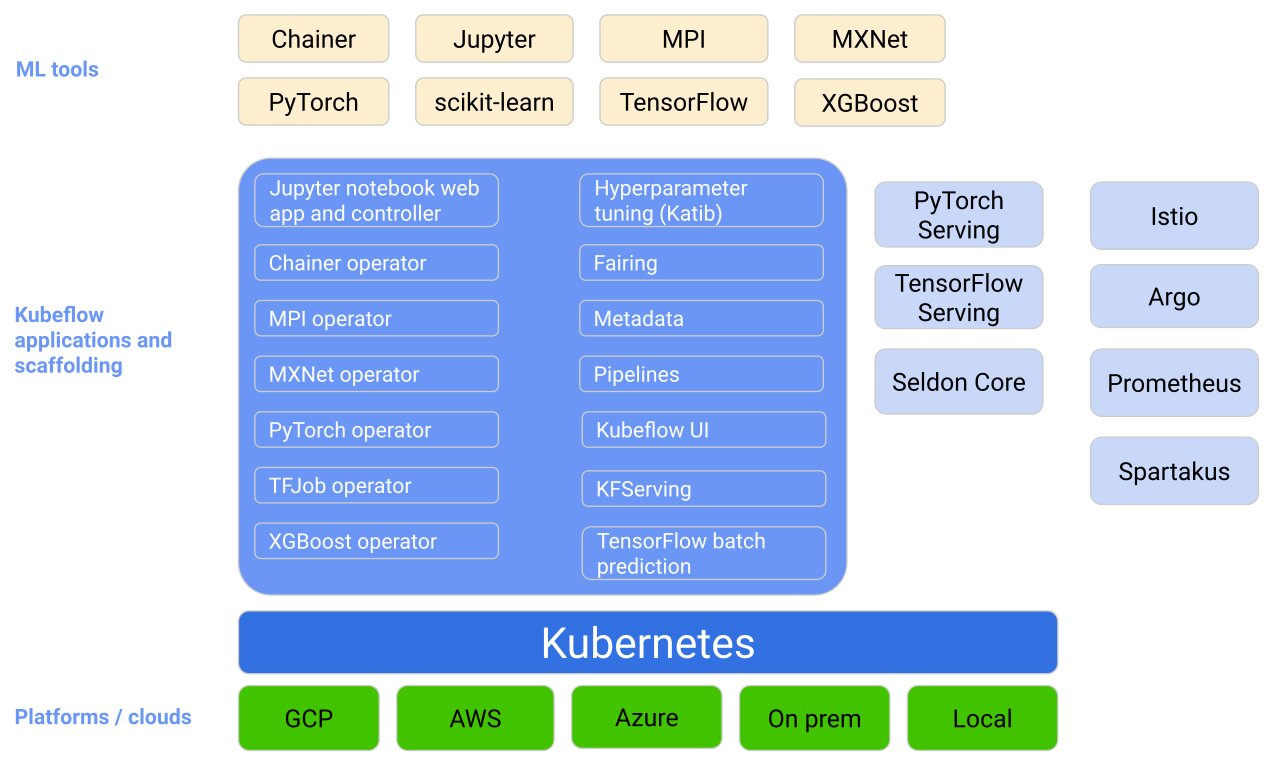
\includegraphics[width=.9\textwidth]{figures/kubeflowaarch}
    \caption{\ Architektúra kubeflow \label{o:latex_friendly_zone}}
\end{figure}

\subsection{Pracovný postup}
Postup pozostáva z viacerých krokov, taktiež z iterácie, ktorá je hlavným prvkom pri vyvíjaní sýtemu strojového učenia. Pri tomto postupe je potrebné vykonávať zmeny v parametroch aby sme dosiahli požadované výsledky.

Následne si povieme niečo viac o týchto postupoch.

Ako prvé by sme mali vyvíjať model na základe predpokladov a testov. Môžeme ho opísať v nasledujúcich bodoch:\cite{web}

\begin{itemize}
    \item Identifikovanie problému, ktorý ma systém vyriešiť 
    \item Zbieranie dát, ktoré potrebujeme na trénovanie modelu
    \item Vyberanie algoritmu a nakódovanie modelu
    \item Experiment s údajmi a trénovanie modelu
	\item Vyladenie parametrov
\end{itemize}

Ďalej môžeme nasadiť systém, ktorý bude vykonávať tieto procesy:

\begin{itemize}
    \item Transformáciu údajov, ktoré náš systém potrebuje
	\item Trénovanie modelu
	\item Podanie modelu na online prevádzku
	\item Monitorovanie výsledkov na úpravu a zmenu modelu
\end{itemize}

\begin{figure}[!ht]
    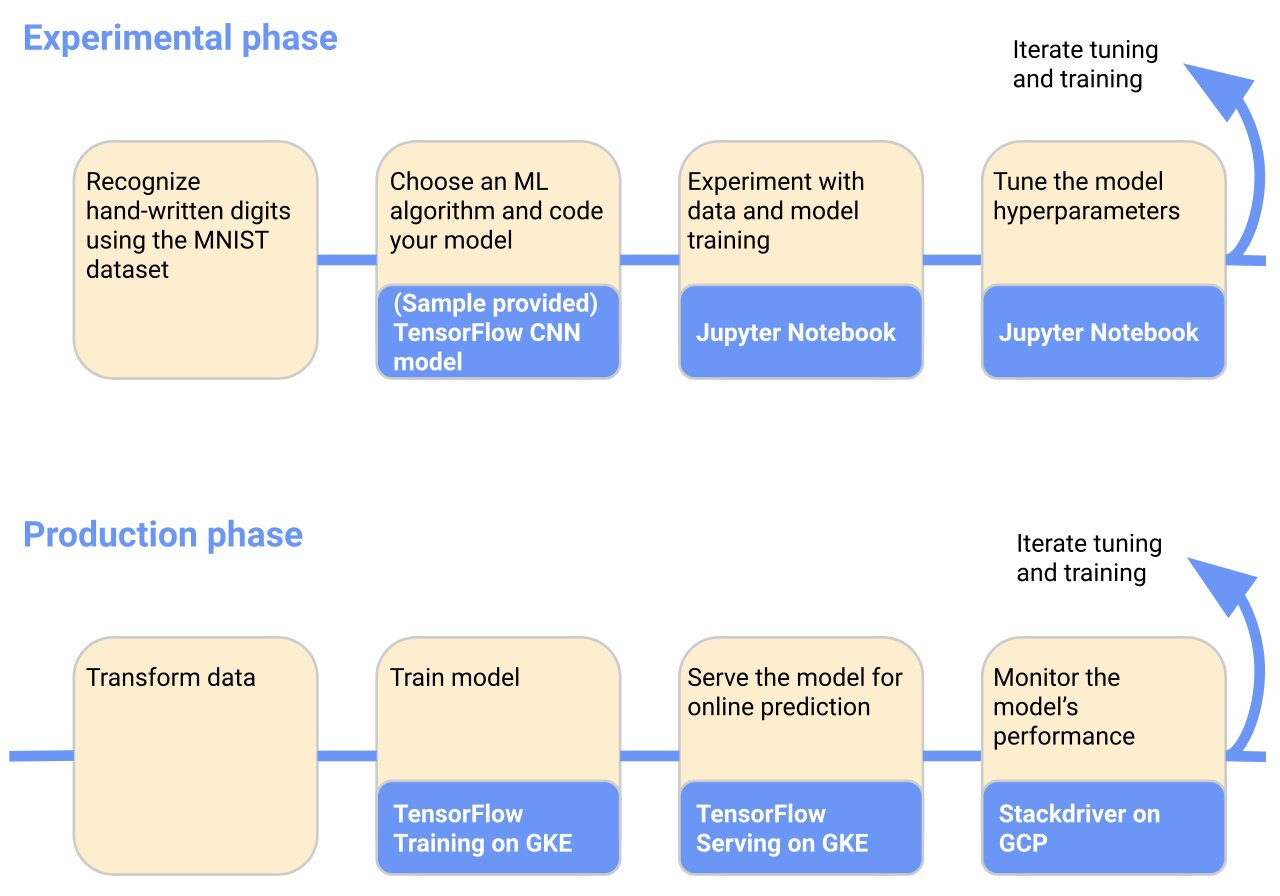
\includegraphics[width=.9\textwidth]{figures/kubeflowwork}
    \caption{\ Pracovné postupy \label{o:latex_friendly_zone}}
\end{figure}

\subsection{Rozhrania}

dopisaaat neskoor

\begin{figure}[!ht]
    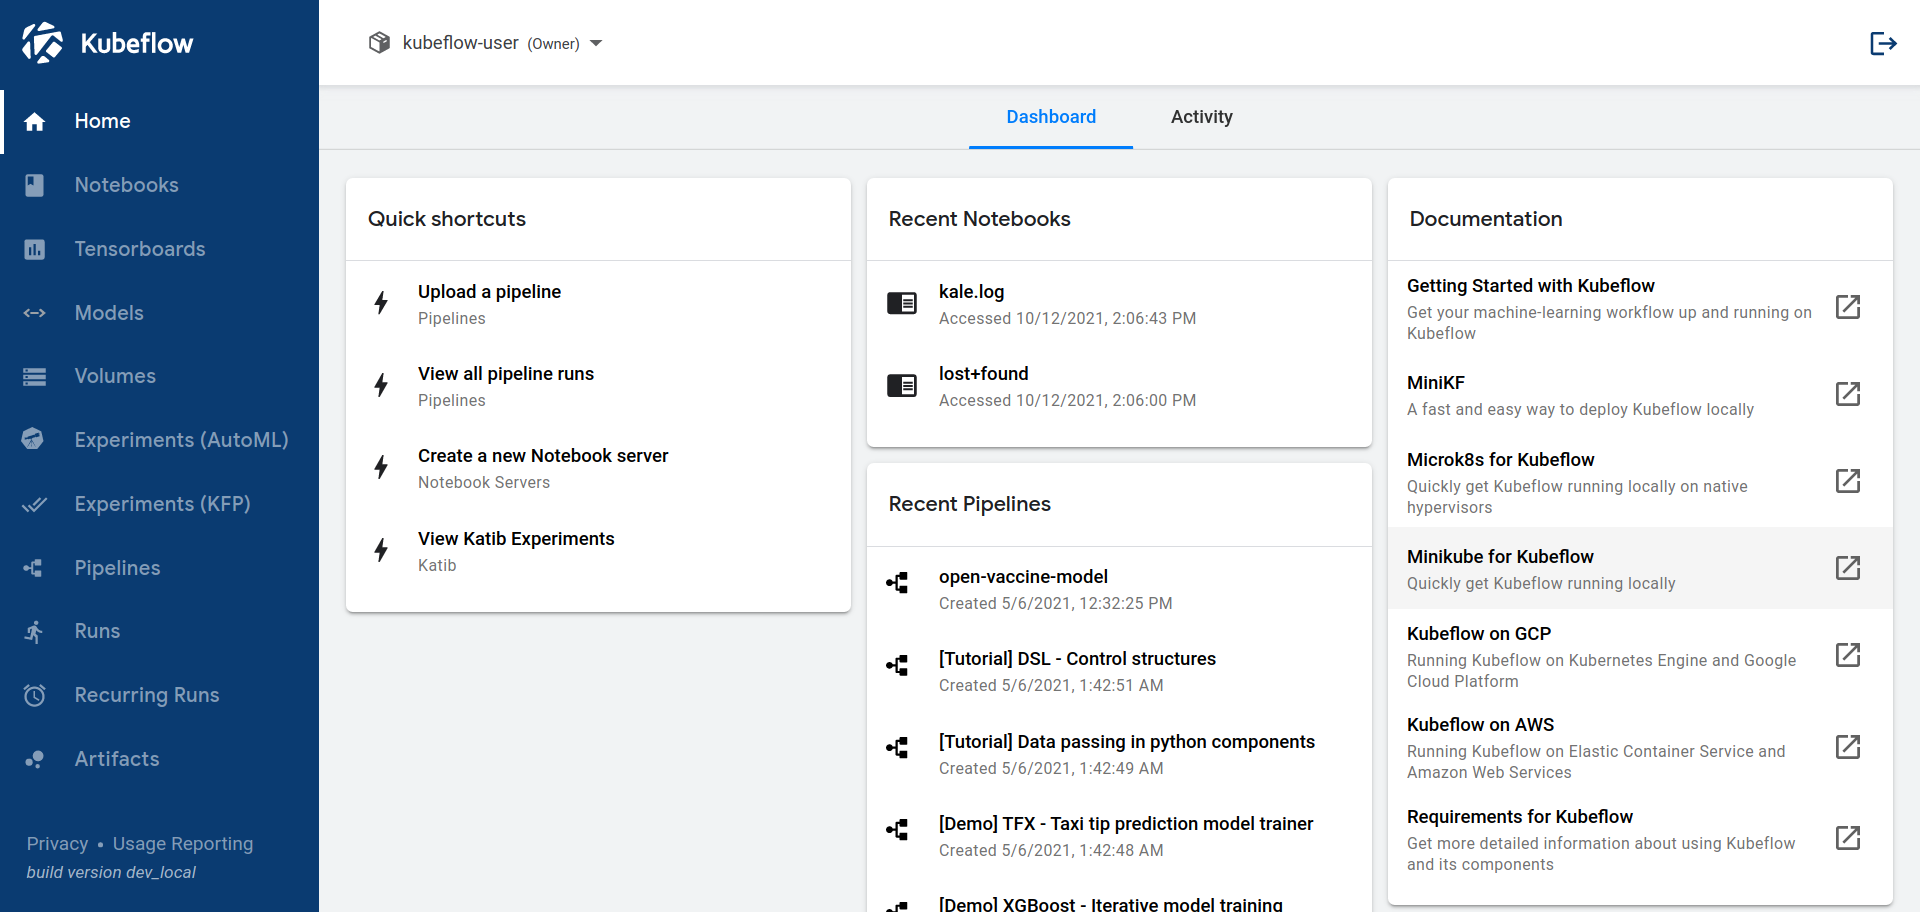
\includegraphics[width=.9\textwidth]{figures/Rozhranie}
    \caption{\ Rozhranie \label{o:latex_friendly_zone}}
\end{figure}

\begin{itemize}
    \item v~knihe \cite{book} autor prezentuje naozaj odvážne myšlienky
    \item nemenej zaujímavé výsledky publikuje ďalší autor v~článku \cite{article} 
    \item v~konferenčnom príspevku \cite{conference} sú uvedené tiež zaujímavé veci
    \item \LaTeX{}\footnote{\url{https://www.latex-project.org/}} je typografický jazyk
\end{itemize}

Given a set of numbers, there are elementary methods to compute its \acrlong{gcd}, which is abbreviated \acrshort{gcd}. This process is similar to that used for the \acrfull{lcm}.

\subsection{Donec vehicula consequat}
\blindtext



\subsection{Nullam in mauris consectetur}
\blindtext

\begin{lstlisting}[language=C,caption={Program, ktorý pozdraví celý svet}]
#include <stdio.h>
int main() {
    /* Print Hello, World! */
    printf("Hello, World!\n");
    return 0;
}
\end{lstlisting}


\subsection{Vestibulum tristique elementum varius}
\blindtext

\begin{table}[!ht]
	\caption{Country list}\label{t:1}
	\smallskip
	\centering

	\begin{tabular}{ |p{3cm}||p{3cm}|p{3cm}|p{3cm}|  }
		\hline
		\multicolumn{4}{|c|}{Country List} \\
		\hline
		Country Name or Area Name& ISO ALPHA 2 Code &ISO ALPHA 3 Code&ISO numeric Code\\
		\hline
		Afghanistan & AF & AFG & 004\\
		Aland Islands & AX & ALA & 248\\
		Albania & AL & ALB & 008\\
		Algeria & DZ & DZA & 012\\
		American Samoa & AS & ASM & 016\\
		Andorra & AD & AND & 020\\
		Angola & AO & AGO & 024\\
		\hline
	\end{tabular}
\end{table}


\section{Phasellus id pretium neque}
\blindtext

\blindtext
